\documentclass[nicefonts,nogruppe,nosemester,noveranstaltung,notutor,noabgabe,utf]{uhb-inf-tex}
\usepackage{url,wrapfig}

\beschreibung{\texttt{\LARGE uhb-inf-tex \normalsize v1.0.1-2009/09/03}}
\zettel{}{}
\gruppe{}{Dominik Menke, \url{dmke@tzi.de}}

\renewcommand\thesection{\arabic{section}}

\begin{document}

\begin{wrapfigure}[17]{r}{.35\linewidth}
	\setlength\fboxsep{0pt}
	\setlength\fboxrule{.01667em}
	\fbox{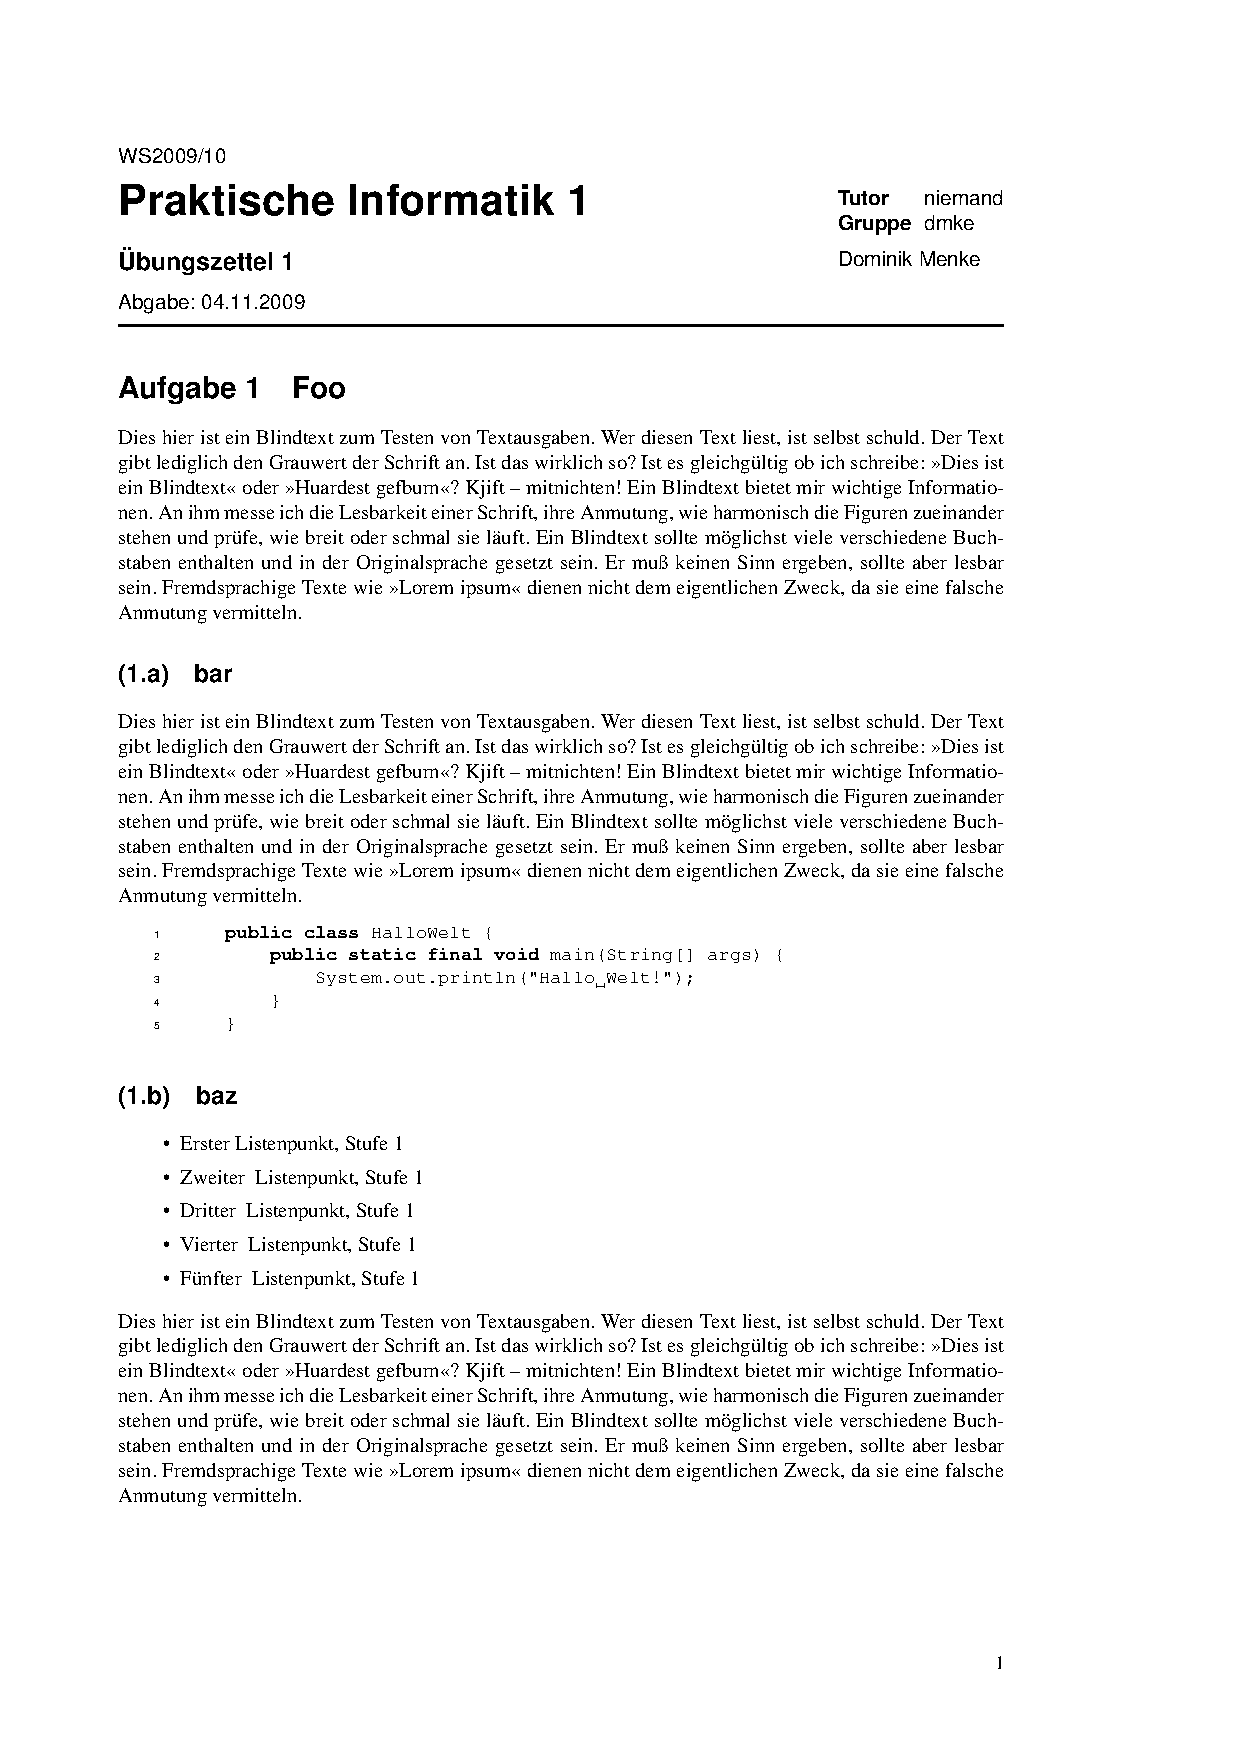
\includegraphics[width=\linewidth]{resources/blindtext.pdf}}
\end{wrapfigure}

\section{Klassen- und Paketbeschreibung}

Die Klasse \texttt{uhb-inf-tex.cls} stellt die Weiterentwicklung der Klasse \texttt{pi1.cls} dar, die wiederum eine von Thomas Röfer adaptierte Version aus \texttt{pi1-muster.cls} und \texttt{defs.tex} war. Nachdem ich mich nun zwei Jahre intensiv mit \LaTeX\ beschäftigt habe, habe ich mir mal die Mühe gemacht einige Dinge auszumerzen, die man so (nicht) mehr macht,\footnote{\url{http://www.ctan.org/tex-archive/info/l2tabu/}} oder anders besser lösen kann. Da mir allerdings die \texttt{pi1.cls} eine große Hilfe beim Lernen von \LaTeX\ war, denke ich ist es nur konsequent, diese Verbesserungen auch an die Erstsemester weiter zu geben.

Herausgekommen ist dabei eine gut anpassbare Dokumentklasse, die sich nicht nur für PI\,1--3, sondern auch für Mathe/Theo/etc. einsetzen lässt.

Im Folgenden seien die Klassenoptionen sowie die bereitgestellten Befehle vorgestellt. Zuvor möchte ich aber die vorausgesetzten und empfohlenen Pakete auflisten.

\subsection{Paketvoraussetzungen}

Es empfiehlt sich immer, ein komplettes und aktuelles \TeX-System zur Verfügung zu haben, und nicht nur den \textit{required}-Teil zu installieren. Letzterer erlaubt eher "`nur"' rudimentären Schriftsatz, abgefahrenere Kommandos sind aber zum Großteil eben nicht enthalten. Bei heutigen Festplattenpreisen sollten 1,5\,GB für Texlive 2008\footnote{\url{http://www.tug.org/texlive/}} nicht schmerzen.

Wer dennoch ein Minimalsystem sein eigen nennt, muss wenigstens diese \LaTeX-Pakete installiert haben:

\begin{itemize}
	\item \texttt{amssymb} -- siehe \url{http://tug.ctan.org/tex-archive/fonts/amsfonts/latex} und \url{http://www.ams.org/tex/amsfonts.html}
	\item \texttt{geometry} -- siehe \url{http://tug.ctan.org/cgi-bin/ctanPackageInformation.py?id=geometry}
	\item \texttt{listings} -- siehe \url{http://tug.ctan.org/cgi-bin/ctanPackageInformation.py?id=listings}
	\item \texttt{fancyhdr} -- siehe \url{http://tug.ctan.org/cgi-bin/ctanPackageInformation.py?id=fancyhdr}
	\item \texttt{enumitem} -- siehe \url{http://tug.ctan.org/cgi-bin/ctanPackageInformation.py?id=enumitem}
	\item Fonts \texttt{mathpazo} und \texttt{beramono}
	\item oder Fonts \texttt{mathptmx}, \texttt{helvet} und \texttt{courier}
	\item oder Font \texttt{lmodern}
\end{itemize}

Daneben werden diese Standardpakete eingebunden (die sowieso immer eingebunden werden sollten):

\begin{itemize}
	\item \texttt{ifthen},
	\item \texttt{inputenc} mit passender Kodierung (siehe unten),
	\item \texttt{babel} mit neuer deutscher Rechtschreibung,
	\item \texttt{fontenc},
	\item \texttt{graphicx},
	\item \texttt{calc},
	\item \texttt{amsmath},
	\item \texttt{textcomp},
	\item \texttt{verbatim}
\end{itemize}

Wie man die einzelnen Pakete nachinstalliert ist sowohl betriebssystem- als auch \TeX"=distributionsspezifisch. Ist ein komplettes \TeX-System eingerichtet, sind die erforderlichen Pakete ebenfalls dabei\dots

\subsection{Klassenoptionen}

Zur schnellen Anpassung gibt es eine Reihe von Optionen, die in der Form

\begin{verbatim}
    \documentclass[option-1,...,option-n]{uhb-inf-tex}
\end{verbatim}

angegeben werden können. Einige sind obligatorisch, ein Fehlen wird durch eine Warnung beim Kompilervorgang bekannt gegeben.

\begin{description}
	\item[Eingabekodierung] Zur Wahl stehen \texttt{utf}, \texttt{mac}, \texttt{win} und \texttt{unix}, die entsprechende Zeichenkodierungen (utf8, applemac, latin15 bzw. latin1) nachladen. Wird keine dieser Optionen angegeben, erscheint der Hinweis, dass man eine eigene Eingabekodierung angeben sollte. Es gibt hier also keinen Default-Wert.
	\item[Schriften] Es stehen drei Schrift-Theman zur Auswahl:
	\begin{enumerate}
		\item Das klassische \LaTeX-Erscheinungsbild mit "`Computer Modern"'-Fonts, bzw. der verbesserten Variante "`Latin Modern"'. Hierzu ist keine Option nötig.
		\item Eine modernere Variante mit Palatino als Brotschrift und Bera Mono als dicktengleiche Schrift für den Quelltext (wie in diesem Dokument). Hierzu gibt es die Option \texttt{nicefonts}.
		\item Als letztes gibt es noch ein "`sparsames"' Thema, das native PDF-Schriften verwendet und so die Dateigröße der PDF signifikant verkleinert. Allerdings sind die mit \texttt{compactfonts} eingestellten Schriften (Helvetica, Times und Courier) nicht sonderlich schön.
	\end{enumerate}
	\item[Anzeige verschiedener Variablen] Wie später noch gezeigt wird, lassen sich einige definierte Variablen entfernen. Im einzelnen sind dies:
	\begin{itemize}
		\item \texttt{notutor} -- unterbindet die Ausgabe des Tutors im Titel und den Kopfzeilen
		\item \texttt{nogruppe} -- "`Gruppe"' plus Nummer werden nicht ausgegeben
		\item \texttt{noabgabe} -- das Abgabedatum erschein nicht
		\item \texttt{nosemester} -- die Semesterangabe wird unterdrückt
		\item \texttt{nobeschreibung} -- die Angabe der Beschreibung ("`Aufgabenblatt"' bzw. "`Lösungsblatt"') wird unterbunden
		\item \texttt{noveranstaltung} -- dies schaltet die Ausgabe der Veranstaltungsbezeichnung aus.
	\end{itemize}
	\item[Verschiedenes]
	Per Default wird unter der Veranstaltungsbezeichnung die Zeichenkette "`Lösungsblatt"' ausgegeben, mit der Option \texttt{aufgabenstellung} wird diese zu "`Aufgabenblatt"' angeändert. Primär ist dies also zur Unterscheidung zwischen Aufgaben und Lösungen zu verstehen.
\end{description}

Die bei diesem Dokument aktiven Optionen lauten:

\begin{verbatim}
    \documentclass[
        nicefonts,
        nogruppe,nosemester,noveranstaltung,notutor,noabgabe,
        utf
    ]{uhb-inf-tex}
\end{verbatim}

\subsection{Befehle und Umgebungen}

Die wichtigsten Befehle zum Einrichten des Titels und der Kopfzeilen sind die folgenden:

\def\cs#1{\char`\\#1}
\def\p#1{$\langle$\textit{#1}$\rangle$}
\def\pb#1{\{\p{#1}\}}

\begin{itemize}
	\item \texttt{\cs{veranstaltung}\pb{kurz}\pb{lang}} -- speichert die Bezeichnung der Veranstaltung; \p{lang} sollte soetwas wie "`Praktische Informatik 1"' sein, während \p{kurz} nur "`PI1"' bekommt.
	\item \texttt{\cs{gruppe}\pb{nummer}\pb{teilnehmer}} -- speichert die Gruppenbezeichnung \p{nummer} sowie die Teilnehmer \p{teilnehmer}. Die Teilnehmer müssen durch \texttt{\cs\cs{}} getrennt sein, z.B. \texttt{\cs{gruppe}\{\$ \cs{alpha}\$\}\{Jane Doe\cs\cs{}Max Mustermann\}}.
	\item Mit \texttt{\cs{zettel}\pb{nummer}\pb{abgabedatum}} kann die Zettel-Bezeichnung gespeichert werden.
	\item \texttt{\cs{semester}\pb{bezeichnung}} speichert das Semester, z.B. \texttt{\cs{semester}\{WS 2009/10\}}.
	\item \texttt{\cs{tutor}\pb{name}} speichert den Namen der Tutorin bzw. des Tutors.
	\item Zur Anpassung der "`Beschreibung"' (also je nach Option "`Aufgabenblatt"' oder "`Lösungsblatt"') kann \texttt{\cs{beschreibung}\pb{beschreibung}} verwendet werden.
\end{itemize}

Daneben gibt es die Umgebung \texttt{Java}, welche Java-Quellcode nicht nur wiedergibt, sondern auch ein wenig aufhübscht. Prinzipiell handelt es sich dabei um eine \texttt{lstlisting}\footnote{Siehe dazu \texttt{listings}-Paket, \url{http://tug.ctan.org/tex-archive/macros/latex/contrib/listings/}}-Umgebung, eben speziell auf Java zugeschnitten. Dieser Umgebung können verschiedene Optionen mitgegeben werden (siehe dazu die Doku), per Default haben alle Listings diese Optionen aktiv:

\begin{lstlisting}[language=tex]
\lstset{
	numbers=left,
	basicstyle=\footnotesize\ttfamily,
	numberstyle=\tiny\sffamily,
	tabsize=4,
	xleftmargin=30pt,
	breaklines=true,
}
\end{lstlisting}

Für die Java-Umgebung ist noch zusätzlich \texttt{language=Java} gesetzt.

\subsection{Ausblick}

Einige Dinge, die noch auf der Todo-Liste stehen sind:

\begin{itemize}
	\item "`Tutorin"' ermöglichen
	\item Haskell für PI3-Vorlagen einbinden
	\item Hinweise für \LaTeX-Anfänger hinzufügen?
	\item Pakete für verschiedene Kurse anlegen (siehe Beispiel \texttt{PI1.cls})
\end{itemize}

\end{document}
